%Theoretical Mechanics Homework_4
\documentclass[10pt,a4paper]{article}
\usepackage[UTF8]{ctex}
\usepackage{bm}
\usepackage{amsmath}
\usepackage{amssymb}
\usepackage{graphicx}
\title{理论力学作业\_4}
\author{陈稼霖 \and 45875852}
\date{2018.11.27}
\begin{document}
\maketitle
\section*{Q1}
\subsection*{(i)}解:
达朗贝尔-拉格朗日方程:
\begin{equation}
\label{dlequ}
\sum_{i=1}^n(\bm{F}_i-m_i\ddot{\bm{r}}_i)\cdot\delta\bm{r}_i = 0
\end{equation}
对于定轴转动的刚体,自由度$s=1$,选取刚体的角位移$\theta$为广义坐标,则虚位移可表示为
\[
\delta\bm{r}_i = \frac{\partial\bm{r}_i}{\partial\theta}\delta\theta = \bm{e}_n\times\bm{r}_i\delta\theta
\]
其中$\bm{e}_n$为与角速度同方向的单位矢量。由于对于刚体上各点,虚角位移$\delta\theta$相等,故方程(\ref{dlequ}) 化为
\[
\sum_{i=1}^n(\bm{F}_i-m_i\ddot{\bm{r}}_i)\cdot(\bm{e}_n\times\bm{r}_i) = 0
\]
其中前一项
\[
\sum_{i=1}^n\bm{F}\cdot(\bm{e}_n\times\bm{r}_i) = \bm{e}_n\cdot\sum_{i=1}^n(\bm{r}_i\times\bm{F}) = M_z
\]
为作用在刚体上所有外力对于定轴的力矩之代数和;

\noindent 后一项
\begin{align*}
\sum_{i=1}^nm_i\ddot{\bm{r}}_i\cdot(\bm{e}_n\times\bm{r}_i) &= \bm{e}_n\cdot\sum_{i=1}^nm_i\bm{r}_i\times\ddot{\bm{r}}_i = \bm{e}_n\cdot\sum_{i=1}^nm_i\bm{r}_i\times(\dot{\bm{\omega}}\times\bm{r}_i)\\
&= \bm{e}_n\cdot\sum_{i=1}^nm_i[\dot{\bm{\omega}}(\bm{r}_i\cdot\bm{r}_i)-\bm{r}_i(\dot{\bm{\omega}}\cdot\bm{r}_i)]\\
&= \bm{e}_n\cdot\sum_{i=1}^nm_iR_i^2\dot{\bm{\omega}} = I_z\dot{\omega}
\end{align*}
其中$R$为刚体上点到轴的直线距离。

\noindent 从而
\[
M_z = I_z\dot{\omega}
\]
即为刚体定轴转动的运动微分方程。
\subsection*{(ii)}解:
达朗贝尔-拉格朗日方程:
\begin{equation}
\label{dlequ2}
\sum_{i=1}^n(\bm{F}_i-m_i\ddot{\bm{r}}_i)\cdot\delta\bm{r}_i = 0
\end{equation}
其中虚位移$\delta\bm{r}_i$可以表示为
\[
\delta\bm{r}_i = \bm{r}_i\times\delta\bm{\theta}
\]
其中虚角位移$\delta\bm{\theta}$为虚角位移,对于刚体上各点,虚角位移$\delta\bm{\theta}$相等,故方程(\ref{dlequ2})化为
\begin{align*}
&\Longrightarrow\sum_{i=1}^n(\bm{F}_i-m_i\ddot{\bm{r}}_i)\cdot\bm{r}_i\times\delta\bm{\theta} = 0\\
&\Longrightarrow\delta\bm{\theta}\cdot\sum_{i=1}^n(\bm{F}_i-m_i\ddot{\bm{r}}_i)\times\bm{r}_i = 0\\
&\Longrightarrow\sum_{i=1}^n(\bm{F}_i-m_i\ddot{\bm{r}}_i)\times\bm{r}_i = 0
\end{align*}
其中前一项
\[
\sum_{i=1}^n\bm{F}\times\bm{r}_i = -\bm{M}
\]
后一项
\begin{align*}
\sum_{i=1}^nm_i\ddot{\bm{r}}_i\times\bm{r}_i &= -\sum_{i=1}^nm_i\bm{r}_i\times\ddot{\bm{r}}_i = -\frac{d}{dt}\sum_{i=1}^nm_i\bm{r}_i\times\dot{\bm{r}}_i+\sum_{i=1}^nm_i\dot{\bm{r}}_i\times\dot{\bm{r}}_i\\
&= -\frac{d}{dt}\sum_{i=1}^nm_i\bm{r}_i\times\dot{\bm{r}}_i\\
&= -\frac{d\bm{J}}{dt}
\end{align*}
从而
\[
\bm{M} = \frac{d\bm{J}}{dt}
\]
即为刚体定点转动时的角动量定理。
\section*{Q2}解:
体系处于纸面所在的二维平面内,且受到$l_1,l_2$两个约束,故自由度为$s=4-2=2$,选取两个广义坐标$\theta_1,\theta_2$。

\noindent 如图(\ref{FigureofHomework_4_Q2})以上杆上端为原点$O$,过$O$竖直方向的直线为$x$ 轴,过$O$水平方向的直线为$y$轴,建立直角坐标系。设分别沿着$x,y$ 轴正方向的单位矢量$\bm{i},\bm{j}$。

\noindent 设上杆质心$A(x_1,y_1)$,下杆质心$B(x_2,y_2)$,则下杆下端$C(x_2+\frac{l_2}{2}\cos\theta,y_2+\frac{l_2}{2}\sin\theta)$。
\begin{figure}[h]
\centering
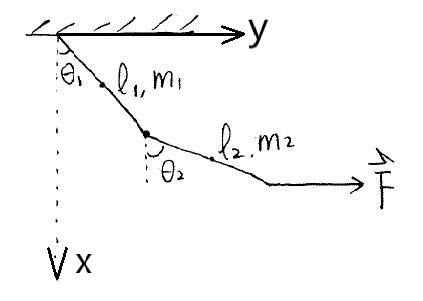
\includegraphics[scale=.5]{FigureofHomework_4_Q2.jpg}\\
\caption{Q2图}\label{FigureofHomework_4_Q2}
\end{figure}

根据虚功原理,体系的平衡条件为
\[
m_1g\delta x_1+m_2g\delta x_2+F\delta(y_2+\frac{l_2}{2}\sin\theta) = 0
\]
约束条件为
\begin{align*}
&f_1 = x_1^2+y_1^2-(\frac{l_1}{2})^2 = 0\\
&f_2 = (x_2-2x_1)^2+(y_2-2y_1)^2-(\frac{l_2}{2})^2 = 0\\
\end{align*}
微分得
\begin{align*}
&\frac{\partial f_1}{\partial x_1} = 2x_1\\
&\frac{\partial f_1}{\partial y_1} = 2y_1\\
&\frac{\partial f_2}{\partial x_1} = 4(2x_1-x_2)\\
&\frac{\partial f_2}{\partial y_1} = 4(2y_1-y_2)\\
&\frac{\partial f_2}{\partial x_2} = 2(x_2-2x_1)\\
&\frac{\partial f_2}{\partial y_2} = 2(y_2-2y_1)
\end{align*}
平衡条件中各项主动力与对应约束条件微分和对应拉格朗日未定乘数的乘积相加等于$0$,并与约束条件联立
\[
\left\{\begin{array}{llllll}
m_1g+\lambda_1\frac{\partial f_1}{\partial x_1}+\lambda_2\frac{\partial f_2}{\partial x_1} = m_1g+2\lambda_1x_1+4\lambda_2(2x_1-x_2) = 0\\
0+\lambda_1\frac{\partial f_1}{\partial y_1}+\lambda_2\frac{\partial f_2}{\partial y_1} = 2\lambda_1y_1+4\lambda_2(2y_1-y_2) = 0\\
m_2g+\lambda_2\frac{\partial f_2}{\partial x_2} = m_2g+2\lambda_2(x_2-2x_1) = 0\\
F+\lambda_2\frac{\partial f_2}{\partial y_2} = F+2\lambda_2(y_2-2y_1) = 0\\
f_1 = x_1^2+y_1^2-(\frac{l_1}{2})^2 = 0\\
f_2 = (x_2-2x_1)^2+(y_2-2y_1)^2-(\frac{l_2}{2})^2 = 0\\
\end{array}\right.
\]
解得
\begin{align*}
&x_1 = -\frac{m_1g+m_2g}{2\lambda_1}\\
&y_1 = -\frac{F}{2\lambda_1}\\
&x_2 = 2x_1-\frac{m_2g}{2\lambda_2}\\
&y_2 = 2y_1-\frac{F}{2\lambda_2}\\
&\lambda_1 = \frac{\sqrt{(m_1+2m_2)^2g^2+F^2}}{l_2}\\
&\lambda_2 = \frac{\sqrt{m^2g^2+F^2}}{l_2}
\end{align*}
约束力为
\begin{align*}
\bm{R}_1 &= \lambda_1\nabla f_1 = \lambda_1(\frac{\partial f_1}{\partial x_1}\bm{i}+\frac{\partial f_2}{\partial y_1}\bm{j}) = \lambda_1(2x_1\bm{i}+2y_1\bm{j})\\
&= \lambda_1(-2\frac{m_1g+m_2g}{2\lambda_1}\bm{i}-2\frac{F}{2\lambda_1}\bm{j})\\
&= -(m_1+m_2)g\bm{i}-F\bm{j}\\
\bm{R}_2 &= \lambda_2\nabla f_2 = \lambda_2(\frac{\partial f_2}{\partial x_2}\bm{i}+\frac{\partial f_2}{\partial y_2}\bm{j}) = \lambda_1(2(x_2-2x_1)\bm{i}+2(y_2-2y_1)\bm{j})\\
&= \lambda_1(-2\frac{m_2g}{2\lambda_2}\bm{i}-2\frac{F}{2\lambda_2}\bm{j})\\
&= -m_2g\bm{i}-F\bm{j}
\end{align*}
综上:上杆在上端铰链处受到的作用力为$= -(m_1+m_2)g\bm{i}-F\bm{j}$,下杆在两杆铰链处受到的相互作用力为$-m_2g\bm{i}-F\bm{j}$
\section*{Q3.}
\subsection*{(1)}解:
如图(\ref{FigureofHomework_4_Q3})以大圆柱体截面圆心为原点$O$,以过$O$竖直直线为$y$ 轴,以过$O$ 点水平直线为$x$轴,建立直角坐标系。设小圆柱体截面圆心$C(x,y)$,小圆柱体相对于处于大圆柱体最低点时所转过的角度为$\varphi$。
\begin{figure}[h]
\centering
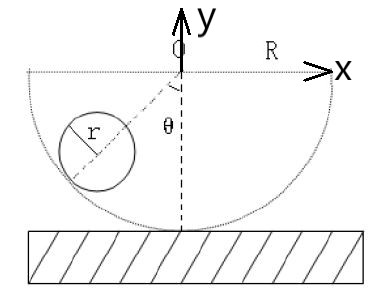
\includegraphics[scale=.5]{FigureofHomework_4_Q3.jpg}\\
\caption{Q3图}\label{FigureofHomework_4_Q3}
\end{figure}

由小圆柱体始终与大圆柱体内表面接触有
\[
x^2+y^2 = (R-r)^2
\]
或写为
\begin{align*}
&x = (R-r)\sin\theta\\
&y = (R-r)\cos\theta
\end{align*}
由小圆柱体始终做纯滚动有
\[
r(\varphi+\theta) = R\theta
\]
综上,小圆柱体的约束方程为
\[
\left\{\begin{array}{lll}
x = (R-r)\sin\theta\\
y = (R-r)\cos\theta\\
r(\varphi+\theta) = R\theta
\end{array}\right.
\]
\subsection*{(2)}答:
小圆柱体的运动属于刚体的平面平行运动,原有三个独立变量,但由(1)有两个约束条件,故自由度为$s=1$。广义坐标取小圆柱体截面圆心和大圆柱体截面圆心连线与竖直方向的夹角$\theta$。
\subsection*{(3)}解:
由(1)中约束方程得
\begin{align*}
&\dot{\varphi} = \frac{R-r}{r}\theta\\
&y = (R-r)\cos\theta
\end{align*}
小圆柱体动能为
\begin{align*}
T &= \frac{1}{2}m(\dot{\varphi} r)^2+\frac{1}{2}(\frac{1}{2}mr^2)\dot{\varphi}^2\\
&= \frac{3}{4}m(R-r)^2\dot{\theta}^2
\end{align*}
以大圆柱体截面圆心处为零重力势能点,小圆柱体的势能为
\[
V = mgy = mg(R-r)\cos\theta
\]
小圆柱体的拉格朗日函数为
\[
L = T-V = \frac{3}{4}m(R-r)^2\dot{\theta}^2-mg(R-r)\cos\theta
\]
小圆柱体的拉格朗日方程为
\begin{align*}
&\frac{d}{dt}(\frac{\partial L}{\partial\dot{\theta}})-\frac{\partial L}{\partial\theta} = 0\\
\Longrightarrow&\frac{3}{2}(R-r)\ddot{\theta}+g\sin\theta = 0
\end{align*}
\subsection*{(4)}解:
由于小圆柱体在平衡位置附近做微小振动,故$\sin\theta\approx\theta$,代入(3)中的拉格朗日方程有
\[
\frac{3}{2}(R-r)\ddot{\theta}+g\theta = 0
\]
解得
\[
\theta = \theta_0\sin(\sqrt{\frac{2g}{3(R-r)}}t+\alpha)
\]
其中积分常数$\theta_0,\alpha$由初始条件决定,小圆柱体的振动频率为$\frac{1}{2\pi}\sqrt{\frac{2g}{3(R-r)}}$。
\section*{Q4.}解:
体系自由度$s=2$,取广义坐标圆环圆心$O$的水平位置坐标$x$和$OC$ 与竖直方向的夹角$\theta$。
体系的动能为
\begin{align*}
T =&\frac{1}{2}m_2\dot{x}^2+\frac{1}{2}(m_2r^2)(\frac{\dot{x}}{r})^2\\
&+\frac{1}{2}m_1[\dot{x}^2+(\dot{\theta}\frac{r}{\sqrt{2}})^2+2\dot{x}\dot{\theta}\frac{r}{\sqrt{2}}\cos\theta]+\frac{1}{2}[\frac{1}{12}m_1(\sqrt{2}r)^2+m_1(\frac{r}{\sqrt{2}})^2]\dot{\theta}^2\\
=&m_2\dot{x}^2+\frac{1}{2}m_1[\dot{x}^2+\frac{7}{6}r^2\dot{\theta}^2+\sqrt{2}r\dot{x}\dot{\theta}\cos\theta]
\end{align*}
设圆环圆心$O$所在高度为零势能,则体系的势能为
\[
V = -m_1g\frac{r}{\sqrt{2}}\cos\theta
\]
体系的拉格朗日函数为
\[
L = T-V = m_2\dot{x}^2+\frac{1}{2}m_1[\dot{x}^2+\frac{7}{6}r^2\dot{\theta}^2+\sqrt{2}r\dot{x}\dot{\theta}\cos\theta]+m_1g\frac{r}{\sqrt{2}}\cos\theta
\]
体系的拉格朗日方程为
\begin{align*}
&\left\{\begin{array}{ll}
\frac{d}{dt}(\frac{\partial L}{\partial\dot{x}})-\frac{\partial L}{\partial x} = 0\\
\frac{d}{dt}(\frac{\partial L}{\partial\dot{\theta}})-\frac{\partial L}{\partial \theta} = 0
\end{array}\right.\\
\Longrightarrow&\left\{\begin{array}{ll}
\frac{d}{dt}(2m_2\dot{x}+m_1\dot{x}+\frac{1}{\sqrt{2}}m_1r\dot{\theta}\cos\theta) = 0\\
\frac{7}{6}r\ddot{\theta}+\frac{1}{\sqrt{2}}\ddot{x}\cos\theta+\frac{1}{\sqrt{2}}g\sin\theta = 0
\end{array}\right.\\
&\text{上式代入下式}\\
\Longrightarrow&\left\{\begin{array}{ll}
\frac{d}{dt}(2m_2\dot{x}+m_1\dot{x}+\frac{1}{\sqrt{2}}m_1r\dot{\theta}\cos\theta) = 0\\
\frac{7}{6}r\ddot{\theta}-\frac{1}{2}\frac{m_1r}{2m_2+m_1}\cos\theta\frac{d}{dt}(\dot{\theta}\cos\theta)+\frac{1}{\sqrt{2}}g\sin\theta = 0
\end{array}\right.\\
&\text{上式直接对$t$积分,下式两边同乘$2\dot{\theta}$并对$t$积分}\\
\Longrightarrow&\left\{\begin{array}{ll}
2m_2\dot{x}+m_1\dot{x}+\frac{1}{\sqrt{2}}m_1r\dot{\theta}\cos\theta = C_1\\
(\frac{7}{6}-\frac{m_1\cos^2\theta}{2(2m_2+m_1)})r\ddot{\theta}-\sqrt{2}g\cos\theta = C_2
\end{array}\right.
\end{align*}
此即该系统的运动微分方程,积分常数$C_1,C_2$由初始条件决定。
\section*{Q5.}解:
体系处于纸面所在的二维平面内,且受到$l_1,l_2$两个约束,故自由度为$s=4-2=2$,选取广义坐标上杆与竖直方向夹角$\theta_1$和下杆与竖直方向夹角$\theta_2$。

\noindent 如图以上杆上端为原点$O$,过$O$竖直方向的直线为$x$轴,过$O$水平方向的直线为$y$轴,建立直角坐标系。设分别沿着$x,y$轴正方向的单位矢量$\bm{i},\bm{j}$。

\noindent 设上杆质心$A(x_1,y_1)$,下杆质心$B(x_2,y_2)$。

\noindent 约束条件为
\begin{align*}
&x_1 = \frac{1}{2}l\cos\theta_1\\
&y_1 = \frac{1}{2}l\sin\theta_1\\
&x_2 = l\cos\theta_1+\frac{1}{2}l\cos\theta_2\\
&y_2 = l\sin\theta_1+\frac{1}{2}l\sin\theta_2
\end{align*}
体系的动能为
\begin{align*}
T =&\frac{1}{2}(\frac{1}{3}ml^2)\dot{\theta}_1^2+\frac{1}{2}m[\dot{x_2}^2+\dot{y_2}^2]+\frac{1}{2}(\frac{1}{12}ml^2)\dot{\theta}_2^2\\
=&\frac{1}{2}(\frac{1}{3}ml^2)\dot{\theta}_1^2+\frac{1}{2}m[(-l\sin\theta_1\dot{\theta}_1-\frac{1}{2}l\sin\theta_2\dot{\theta}_2)^2+(l\cos\theta_1\dot{\theta}_1+\frac{1}{2}l\cos\theta_1\dot{\theta}_2)^2]\\
&+\frac{1}{2}(\frac{1}{12}ml^2)\dot{\theta}_2^2\\
=&ml^2[\frac{2}{3}\dot{\theta}_1^2+\frac{1}{6}\dot{\theta}_2^2+\frac{1}{2}(\sin\theta_1\sin\theta_2+\cos\theta_1\cos\theta_2)\dot{\theta}_1\dot{\theta}_2]\\
=&ml^2[\frac{2}{3}\dot{\theta}_1^2+\frac{1}{6}\dot{\theta}_2^2+\frac{1}{2}\cos(\theta_2-\theta_1)\dot{\theta}_1\dot{\theta}_2]
\end{align*}
由此
\begin{align*}
&\frac{\partial T}{\partial\dot{\theta}_1} = ml^2[\frac{4}{3}\dot{\theta}_1+\frac{1}{2}\cos(\theta_2-\theta_1)\dot{\theta}_2]\\
\Longrightarrow&\frac{\partial T}{\partial\dot{\theta}_1}|_{0} = 0,~~~~\frac{\partial T}{\partial\dot{\theta}_1}|_{\Delta t}=ml^2[\frac{4}{3}\dot{\theta}_1+\frac{1}{2}\dot{\theta}_2]\\
&\frac{\partial T}{\partial\dot{\theta}_2} = ml^2[\frac{1}{3}\dot{\theta}_2+\frac{1}{2}\cos(\theta_2-\theta_1)\dot{\theta}_1]\\
\Longrightarrow&\frac{\partial T}{\partial\dot{\theta}_2}|_{0} = 0,~~~~\frac{\partial T}{\partial\dot{\theta}_2}|_{\Delta t} = ml^2[\frac{1}{3}\dot{\theta}_2+\frac{1}{2}\dot{\theta}_1]
\end{align*}
冲量$I$可以表示为
\[
\bm{I} = \int_0^{\Delta t}\bm{F}dt
\]
广义冲量为

\begin{align*}
I_{\theta_1} =&\int_0^{\Delta t}\frac{\partial[l(\cos\theta_1+\cos\theta_2)\bm{i}+l(\sin\theta_1+\sin\theta_2)\bm{j}]}{\partial\theta_1}\bm{F}dt\\
=&\int_0^{\Delta t}lF\cos\theta_1dt\\
=&lI\\
I_{\theta_2} =&\int_0^{\Delta t}\frac{\partial[l(\cos\theta_1+\cos\theta_2)\bm{i}+l(\sin\theta_1+\sin\theta_2)\bm{j}]}{\partial\theta_2}\bm{F}dt\\
=&\int_0^{\Delta t}lF\cos\theta_2dt\\
=&lI
\end{align*}
瞬时力作用下的拉格朗日方程
\begin{align*}
&\frac{\partial T}{\partial\dot{\theta_1}}|_{\Delta t}-\frac{\partial T}{\partial\dot{\theta_1}}|_{0} = I_{\theta_1} = lI\\
&\frac{\partial T}{\partial\dot{\theta_2}}|_{\Delta t}-\frac{\partial T}{\partial\dot{\theta_2}}|_{0} = I_{\theta_2} = lI
\end{align*}
解得碰后上下两杆的角速度分别为
\begin{align*}
&\omega_1 = \dot{\theta_1} = -\frac{6}{7}\frac{I}{ml}\\
&\omega_2 = \dot{\theta_2} = \frac{30}{7}\frac{I}{ml}
\end{align*}
其中正号代表逆时针方向,负号代表顺时针方向。
\end{document}
